
\chapter[A Proposta]{A PROPOSTA}

A proposta deste trabalho é criar uma plataforma, denominada Gamifier, de apoio a construção de projetos de gamificação, capaz de exportar projetos para o Funifier. A plataforma servirá para automatizar o processo de criação dos projetos. Com a ambição de simplificar e incentivar a inserção de gamificação no cotidiano das pessoas que tem interesse pelo tema.

 Este capítulo está estruturado da seguinte maneira, a seção 1 é a introdução, onde é feita uma contextualização sobre o porque de se construir o Gamifier com tal propósito e a seção 2, construção da plataforma, onde é descrito o processo de construção da ferramenta.           

\section{Introdução}

Ninguém tem que jogar um jogo, as pessoas tem que trabalhar e pagar sua contas, elas não são obrigadas a jogar, mas jogam \cite{chou2015actionable},  \cite{mcgonigal2011reality}. E se sentem motivadas, felizes e incentivadas quando estão jogando. O jogo gera mais esperança de sucesso nas pessoas, em comparação ao jogos, a realidade não demonstra esperança \cite{mcgonigal2011reality}.

As pessoas têm tanto interesse em jogar e não dispõem do mesmo interesse para realizar tarefas cotidianas ou conquistar uma meta a longo prazo. 
A proposta de construção de uma ferramenta com o intuito de inserir gamificação na vida das pessoas vem para facilitar o preenchimento desta lacuna. A construção de uma plataforma que dê suporte a criação de projetos pode vir a auxiliar quanto a aplicação, na vida real, da motivação intrinsecamente ligada aos jogos. Um sistema que proporcione a criação de projetos de gamificação motivadores.

Há algumas décadas têm-se estudado a motivação intrinsecamente ligada ao jogo e como aplicá-la em outras áreas com o mesmo sucesso. Motivar apenas não basta, motivação acaba, é preciso pensar maneiras de manter a motivação. Criar um ciclo onde além de motivadas as pessoas permaneçam disciplinadas, não por obrigação, e sim porque sentem vontade de sempre seguir adiante. 

A proposta é criar uma plataforma de apoio  a criação de projetos de gamificação. A ferramenta existirá para que o processo de criação de proejtos de gamificação seja feito de maneira mais descomplicada. Pretende-se também que com o uso do Gamifier, o usuário com algum grau de conhecimento relacionado ao assunto tenha sua produtividade elevada no momento da construção do projeto. 

\section{Construção do Gamifier}

A Fig. (\ref{fig01}) representa os componentes internos que serão utilizados para dar forma ao gamifier, o cubo representa as unidades principais, as técnicas de gamificação e os atributos das técnicas de gamificação, dando forma ao \textit{core} da ferramenta.

\begin{figure}[h]
	\centering
		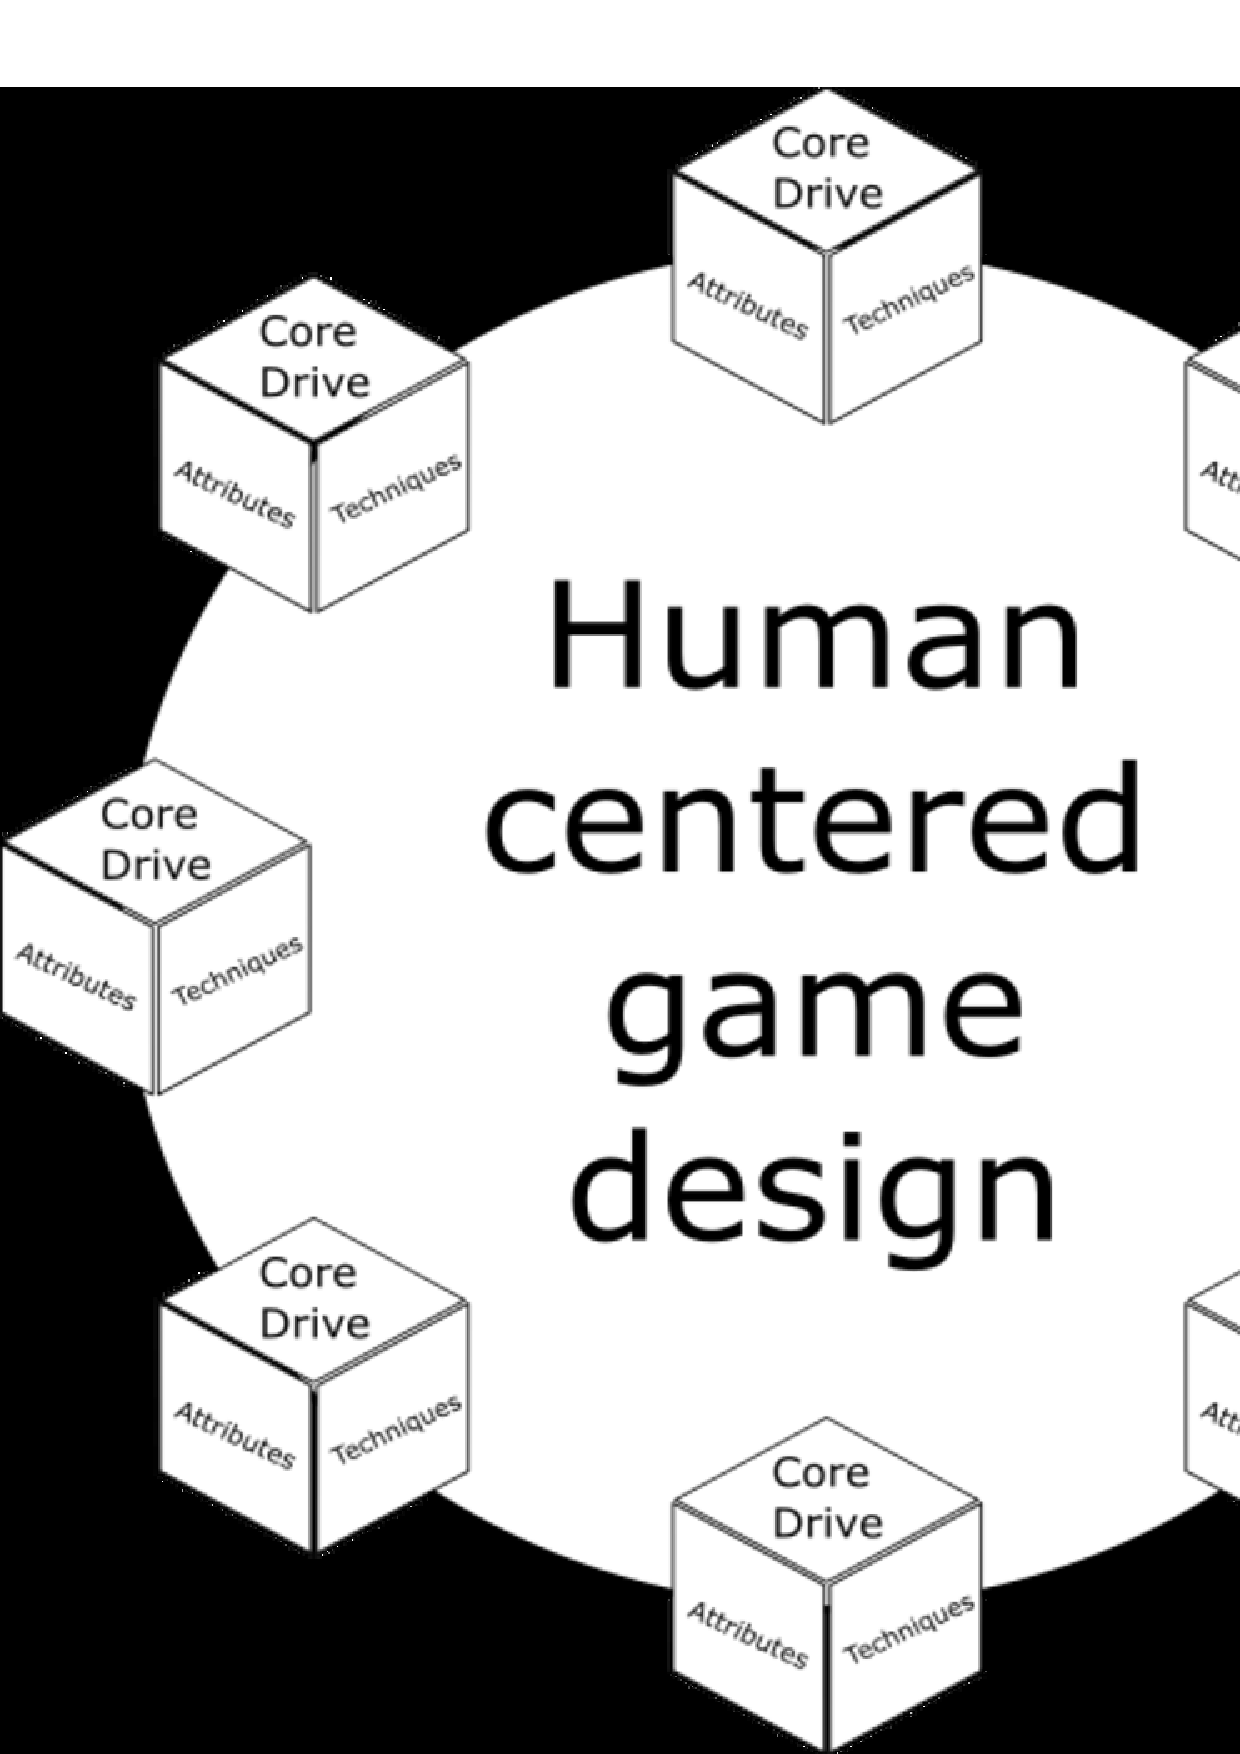
\includegraphics[keepaspectratio=true,scale=0.5]{figuras/hcgd.png}
	\caption{Composição da Ferramenta.\label{fig01}}
\end{figure}


A a parte superior do cubo, são as unidades principais do \textit{framework}, as técnicas de gamificação, representadas como o lado direito do cubo, compõem as unidades principais, os atributos, representados como o lado esquerdo do cubo, compõem as técnicas de gamificação. 

A plataforma tem como propósito o apoio a construção de projetos gamificação que motivem os seus usuários e ela terá o usuário como foco, o \textit{design} focado no ser humano \cite{chou2015actionable} ou \textit{design}  centrado no usuário \cite{kumar2013gamification}.


O  \textit{framework} Octalysis, modelo proposto por \cite{chou2015actionable} , foi escolhido como alicerce para a construção da ferramenta.
Uma abstração do Octalysis para visualizar como se daria a implementação foi realizada e foi possível perceber que as unidades principais do \textit{framework} juntamente com as técnicas de gamificação existentes estão bem alinhadas com o principal proposito da ferramenta. 

Chou utiliza as unidades principais do \textit{framework} para motivar os usuários e as técnicas de gamificação para representar elementos de jogos. As técnicas possuem mais de uma função, são utilizadas também para intensificar a motivação representada pela unidade principal da qual fazem parte. O emprego correto das mesmas na construção do projeto produz um resultado mais satisfatório. Como gamificação é o ato de aplicar elementos de jogos em contexto fora de jogo, as técnicas de gamificação representam a ligação entre o contexto de não jogo ao contexto de jogo. 

As oito unidades principais do Octalysis possuem uma descrição e são compostas por inúmeras técnicas de gamificação. As técnicas de gamificação possuem uma descrição, mas não é especificado qual a sua composição.  Para construir o Gamifier definiu-se então um conjunto de atributos irão compor as técnicas. Além de construir uma plataforma, a proposta é construir uma plataforma que faça uso dessa extensão proposta ao \textit{framework}.

Atualmente não há uma definição formal de um conjunto mínimo de atributos que devem estar presentes para que uma técnica seja implementada corretamente. Não havia um mapeamento que informasse ao construtor do projeto de gamificação como as técnicas se relacionam. Se é possível implementar todas de uma vez, se a implementação de uma afeta a implementação de outra. Não há uma definição de como deve ser o relacionamento entre as técnicas de gamificação. Isso acarreta uma dificuldade para identificar se o projeto está sendo construído corretamente. 

Afim obter a relação das técnicas entre si e das técnicas entre as unidades principais foi realizado o mapeamento das técnicas de gamificação. Inicialmente levantou-se as UPs e as técnicas de gamificação pertencentes a elas. Porém, a primeira fonte de informação não continha todas as técnicas de gamificação presente no Octalysis. A busca foi estendida a outros meios.

 Cada técnica é composta por um identificador representado por uma \#, seguido de um número, como a técnica de número \#10 narrativa, por exemplo.  As técnicas possuem ainda uma descrição, para facilitar o entendimento da mesma. Atualmente além das oito unidades principais foram mapeadas cerca de noventa técnicas de gamificação.

As técnicas de gamificação tem uma descrição simples e intuitiva. É fácil entender o que a técnica faz e o que ela pretende motivar no usuário. Porém essa informacão provem de um conhecimento muito atrelado a experiência pessoal de quem propôs a existência e o uso da técnica. Quando se faz necessário realizar a implementação, tirar do campo das idéias e colocar em prática, esse conhecimento teórico não é suficiente, porque está muito ligado ao conhecimento adquirido ao longo dos anos pelo especialista em gamificação e nem todos são especialistas.

 A proposta aqui é justamente tornar a gamificação acessível também a não especialistas. Para tornar a implementação das técnicas mais tangível, foi definido um conjunto de atributos caracterizadores. A intenção é que eles tornam as técnicas de gamificação passíveis de implementação sem que elas percam a identidade ou o foco principal pertencentes a elas e gerar uma extensão do Octalysis.

 O conjunto de atributos definidos para compor a estrutura interna das técnicas são alguns dos indicadores de engajamento definidos por \cite{fredericks2004school}. Os autores dividem, como mencionado no capítulo 2, os engajamentos em três tipos, o engajamento emocional, que trata, por exemplo, de emoções como alegria, interesse e raiva.  O engajamento comportamental, que trata de indicadores de conduta, tais como, esforço, atenção e persistência. O engajamento cognitivo, que trata, por exemplo, de flexibilidade para resolver um problema, concentração e domínio.

 Engajamento também pode ser interpretado neste contexto como envolvimento. Cada tipo de engajamento possui alguns indicadores, os indicadores caracterizam os tipos de engajamento e foram escolhidos aqui também para caracterizar as técnicas de gamificação. 

 Os indicadores foram pensados como adjetivos caracterizando as técnicas de gamificação. A estrutura interna das técnicas é igual, independente da técnica de gamificação em questão e foi pautada em aspectos educacionais, outros aspectos não foram levados em consideração para o TCC1 . Os indicadores escolhidos para compor a estrutura interna das técnicas são: 


\begin{itemize}
\item  \textbf {Envolvimento com o trabalho:}  Mensura a quantidade de envolvimento com a gamificação que a técnica exigirá do usuário.
\item  \textbf {Participação:}  Mensura quanta participação efetiva na gamificação a técnica exigirá do usuário
\item  \textbf {Atenção:}  Mensura quanta atenção a gamificação exigirá do usuário.
\item  \textbf {Persistência:} Mensura quão persistente o usuário será para obter resultados no projeto de gamificação. 
\item  \textbf {Domínio:} Mensura a quantidade de maestria que o usuário precisará dispor para executar a técnica de gamificação. 
\item  \textbf{Social:} Mensura a quantidade de envolvimento social que a técnica dispõe para o usuário e quão social a técnica pode ser.
\end{itemize}


Cada indicador representará um atributo da técnica de gamificação e receberá uma valor que representa o grau de pertinência à técnica de gamificação, os valores variam de um a cinco e serão concedidos de acordo com a escala de Likert. A escala de Likert utilizada possui cinco itens: 

\begin{itemize}
\item  \textbf {Nota 1 - Muito aquém:} O atributo influência fracamente a técnica de gamificação
\item  \textbf {Nota 2 - Aquém:} O atributo influencia aquém do normal a técnica de gamificação
\item  \textbf {Nota 3 - Suficiente / Normal:} O atributo influencia de forma suficiente (normal) a técnica de gamificação
\item  \textbf {Nota 4 - Além:} O atributo influência além da normal a técnica de gamificação
\item  \textbf {Nota 5 - Muito além:} O atributo influencia plenamente a técnica de gamificação
\end{itemize}


A Fig. (\ref{fig02}) é um exemplo de pontuação de atributos para a técnica número 10, a narrativa, cada coluna representa uma das notas da escala, a figura conta com a menor nota e a maior nota como exemplo nas extremidades da tabela.

\begin{figure}[h]
	\centering
		\includegraphics[keepaspectratio=true,scale=0.5]{figuras/notas.png}
	\caption{Representação dos atributos pontuados\label{fig02}}
\end{figure}

\newpage


A Fig. (\ref{fig03}) representa a composição da estrutura da ferramenta. Cada unidade principal é composta por suas técnicas de gamificação. A unidade principal utilizada como exemplo é a significado épico e chamado. A figura apresenta algumas das técnicas de gamificação pertencentes a esta unidade, como \#10 narrativa, \#23 sorte de iniciante, \#26 elitismo e \#27 herói da humanidade. 

Cada técnica é composta por seis atributos e cada atributo recebe uma nota de um a cinco. Os atributos têm duas funções, caracterizar as técnicas de gamificação e espelhar o envolvimento do usuário com a gamificação. Por exemplo, se a técnica exige do usuário muita atenção e persistência a gamificação também exigirá. 

Com a definição dos atributos formadores das técnicas é possível visualizar a estrutura interna da ferramenta em si. A ferramenta será composta da unidades principais do Octalysis, das técnicas de gamificação e dos atributos das técnicas, os indicadores de engajamento. 


\begin{figure}[h]
	\centering
		\includegraphics[keepaspectratio=true,scale=0.25]{figuras/mapeamento.png}
	\caption{Estrutura geral da ferramenta.\label{fig03}
}
\end{figure}


Após ser feito o mapeamento de todas as técnicas de gamificação existentes no \textit{framework} é necessário mapear a ligação entre as mesmas. O mapeamento das técnicas já foi realizado e todos os indicadores receberam os valores pertinentes. O próximo passo é identificar se existe ligação entre as técnicas  e se a implementação de uma pode exercer influência positiva ou negativa sobre  outra.. O mapeamento inicial gerou uma estrutura similar a Fig (\ref{fig04}).

\begin{figure}[h]
	\centering
		\includegraphics[keepaspectratio=true,scale=0.5]{figuras/hierarquia.png}
	\caption{Hieraquia dos elementos da ferramenta.	\label{fig04}}
\end{figure}

A Fig. (\ref{fig04}) representa o relacionamento proposto entre as unidades principais, representadas na figura como \#XUP. As técnicas de gamificação como \#número e os atributos das técnicas de gamificação, A. Os componentes estão distribuídos de forma hierárquica, mas a abordagem não necessariamente seguirá essa restrição.  O usuário poderá escolher a forma como irá montar o projeto, o projeto poderá ser iniciado pelas técnicas de gamificação e as inter-relações entre as técnicas de gamificação não são necessariamente hierárquicas.

A Fig. (\ref{fig05}) representa o relacionamento entre as técnicas de gamificação, esse inter-relacionamento também ocorrerá entre as unidades principais, se a técnica de gamificação que pertence a uma determinada unidade principal interage diretamente com uma técnica pertencente a outra unidade, as unidades acabam formando uma relação indireta. 

A Fig. (\ref{fig05}) demonstra como funcionará o relacionamento entre as técnicas e entre as unidades principais. Como as técnicas possuem o mesmo conjunto de atributos, quando atributos de diferentes técnicas possuem valores parecidos, infere-se que eles despertam no usuário da gamificação as mesmas motivações ou níveis muito próximos de motivação, apesar de serem técnicas diferentes, dessa maneira se dará a construção do relacionamento entre as mesmas, nem todas as técnicas se relacionam e nem todas que se relacionam fazem isso da mesma maneira, nem com a mesma intensidade.

A Fig. (\ref{fig05}) representa como se dará a o relacionamento entre as técnicas e as unidades principais, \#1UP e \#2UP são as unidades principais e os números seguidos de \# são as técnicas de gamificacão e as linhas representam o relacionamento entre os elementos. Apesar de não estarem presentes visualmente, os atributos também fazem parte deste relacionamento.

Como indica a figura, o relacionamento entre as técnicas forma um grafo, onde as técnicas de gamificação e as unidades principais são os vértices e as arestas a ligação entre estes elementos. Quando uma unidade principal está ligada a uma técnica que está ligada a outra unidade principal existe uma relação indireta entre as unidades principais, essa ligação, por exemplo, é representada na figura como relacionamento indireto entre a \#1UP, técnica \#23 e \#2UP. E este relacionamento é que será responsável por indicar a consistência do projeto, como o relacionamento está mapeado internamente, quando o usuário criar um projeto que não está consistente com o relacionamento das técnicas e unidades principais ele será informado.

\begin{figure}[h]
	\centering
		\includegraphics[keepaspectratio=true,scale=0.5]{figuras/grafo.png}
	\caption{Relacionamento entre os elementos da ferramenta.\label{fig05}}
\end{figure}



